
\documentclass[9pt]{beamer}

\usepackage[latin1]{inputenc}
\usepackage{colortbl}
\usepackage[english]{babel}

\pgfdeclareimage[height=1.5cm]{alice-logo}{alice-logo}
\logo{\pgfuseimage{alice-logo}}

\newcommand{\myblue} [1] {{\color{blue}#1}}
\newcommand{\newauthor}[4]{
  \parbox{0.26\textwidth}{
    \texorpdfstring
      {
        \centering
        #1 \\
        \myblue{{\href{#2}{\texttt{#3}}}} \\
        #4 \\
      }
      {#1}
  }
}


% for code colouring
\usepackage{minted}
\definecolor{bg}{rgb}{0.95,0.95,0.95}
\setminted{bgcolor=bg}

% beamer template
\beamertemplatetransparentcovereddynamic
\usetheme{Binet}

\hypersetup{%
	pdftitle={Exploring polyglot software frameworks in ALICE with FairMQ and fer},%
   pdfauthor={Sebastien Binet},%
  pdfauthor={Laurent Aphecetche},%
%
}

\title[FairMQ and fer]{Exploring polyglot software frameworks in ALICE\\ with \tt{FairMQ} \& \texttt{fer}}
\date{2018-07-09}
\author[S.Binet \& L. Aphecetche]{
 \parbox{0.26\textwidth}{
	\texorpdfstring
	  {
		\centering
 		Sebastien Binet \\
 		CNRS/IN2P3/LPC \\
		\myblue{\href{mailto:binet@cern.ch}{\texttt{binet@cern.ch}}} \\
 	  }
	{Sebastien Binet}
}
 \and %
 \parbox{0.26\textwidth}{
	\texorpdfstring
	  {
		\centering
 		Laurent Aphecetche \\
 		CNRS/IN2P3/Subatech \\
 		\myblue{\href{mailto:laurent.aphecetche@cern.ch}{\texttt{laurent.aphecetche@cern.ch}}} \\
 	  }
	{Laurent Aphecetche}
}
 }
\institute[ALICE]{\insertlogo\hskip0.1cm}


\begin{document}

\frame{\titlepage
\begin{center}
CHEP-2018
\end{center}
}

\part<presentation>{Main Talk}

\section[slides]{slides}

\begin{frame}[fragile]
\frametitle{AliceO2}


ALICE is working on a new software framework for the O2 project:


\begin{itemize}
\item a new framework to tackle the challenges of Run-3 data taking
\item a new framework that brings together Online and Offline
\item a new framework that builds upon \myblue{\href{https://github.com/FairRootGroup/FairRoot}{\texttt{FairRoot}}} and \myblue{\href{https://github.com/FairRootGroup/FairMQ}{\texttt{FairMQ}}}
\end{itemize}


	\begin{exampleblock}{}
\begin{verbatim}
The FairRoot framework is an object oriented simulation, reconstruction
and data analysis framework.
It includes core services for detector simulation and offline analysis
of particle physics data.
FairRoot is the standard simulation, reconstruction and data analysis
framework for the FAIR experiments at GSI Darmstadt.
\end{verbatim}
	\end{exampleblock}{}



\end{frame}

\begin{frame}[fragile]
\frametitle{FairMQ}


FairMQ (\myblue{\href{https://indico.cern.ch/event/587955/timetable/?view=standard\#454-alfa-alice-fair-new-messag}{\texttt{\#454}}}) is a distributed processing toolkit, written in \texttt{C++}, with pluggable transports (\texttt{ZeroMQ}, \texttt{nanomsg}).


\begin{figure}[h]
\begin{center}
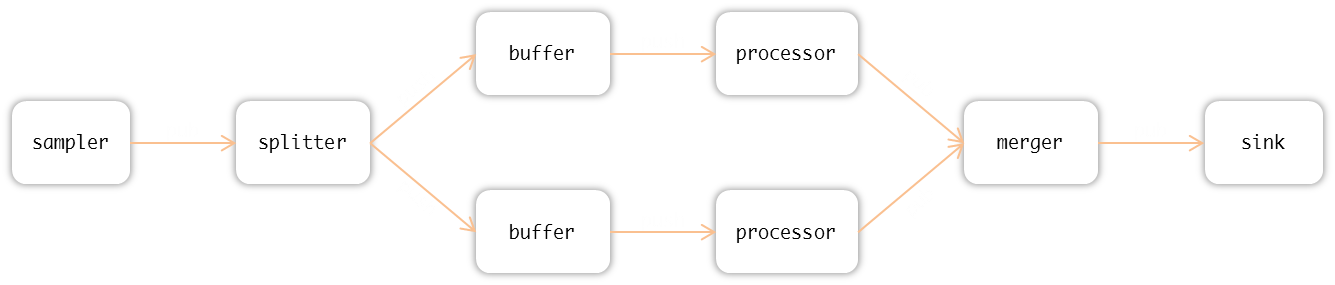
\includegraphics[width=10cm,height=2cm]{_figs/fairmq-example-topology.png}
\end{center}

\end{figure}

Each box can be a different process, possibly on a different remote machine.
This architecture enables a much smoother \textbf{horizontal} \textbf{scaling} when data taking or data processing demands it.


Each box may be connected to another via various protocols: \texttt{tcp}, \texttt{udp}, \texttt{ipc}, \texttt{inproc}, shared-memory.



\end{frame}

\begin{frame}[fragile]
\frametitle{FairMQ}


FairMQ has a concept of \texttt{Devices} which are executed and connected together to form various topologies:



\begin{minted}[]{c++}
class FairMQDevice : <...> {
public:
 int
 Send(const std::unique_ptr<FairMQMessage>& msg,
      const std::string& chan, const int i) const;

 int
 Receive(const std::unique_ptr<FairMQMessage>& msg,
         const std::string& chan, const int i) const;

protected:
  virtual void Init();    virtual void InitTask();
  virtual void Run();
  virtual bool ConditionalRun();
  virtual void Pause();
  virtual void Reset();   virtual void ResetTask();
};
\end{minted}


Users are supposed to \textbf{at} \textbf{least} override \texttt{FairMQDevice::Run()}.



\end{frame}

\begin{frame}[fragile]
\frametitle{FairMQ}


Topologies can be created and described via \texttt{JSON} files (or XML, or via DDS (see \myblue{\href{https://indico.cern.ch/event/587955/timetable/?view=standard\#407-dds-the-dynamic-deployment}{\texttt{\#407}}})):


\begin{minted}[fontsize=\small]{json}
{
    "fairMQOptions":
    {
        "devices":
        [{
            "id": "sampler1",
            "channels":
			[{
                "name": "data1",
                "sockets":
				[{
                    "type": "push",
                    "method": "bind",
                    "address": "tcp://*:5555",
                    "sndBufSize": 1000,
                    "rcvBufSize": 1000,
                    "rateLogging": 0
                }]
            }]
        },
[...]
}

\end{minted}


\end{frame}

\begin{frame}[fragile]
	\frametitle{\tt{fer}}


As FairMQ is distributed with each device talking over \texttt{ZeroMQ} or \texttt{nanomsg}, one can write each device in any language (which has support for \texttt{nanomsg} or \texttt{ZeroMQ}).


\texttt{\$OTHER\_LANGUAGE} could be:


\begin{itemize}
\item \texttt{Java}
\item \texttt{Perl}
\item \texttt{Python}
\item \texttt{Rust}
\item ... 
\end{itemize}

or even just \texttt{bash} + \texttt{netcat} :)


Let's do that in \myblue{\href{https://golang.org}{\texttt{Go}}}.



\end{frame}

\begin{frame}[fragile]

	\begin{columns}
		\begin{column}{0.49\textwidth}
			\begin{block}{}
				\begin{center}
				Interlude: \texttt{Go}
				\end{center}
			\end{block}

\begin{figure}[h]
\begin{center}

\includegraphics[width=\textwidth]{_figs/golang-logo.png}
\end{center}

\end{figure}

		\end{column}
	\end{columns}


\end{frame}

\begin{frame}[fragile]
\frametitle{Elements of Go}


\begin{itemize}
\item Russ Cox, Robert Griesemer, Ian Lance Taylor, Rob Pike, Ken Thompson
\end{itemize}

\begin{itemize}
\item \textbf{Concurrent}, \textbf{garbage-collected}
\item An Open-source general progamming language (BSD-3)
\item feel of a \textbf{dynamic} \textbf{language}: limited verbosity thanks to the \emph{type} \emph{inference} \emph{system}, map, slices
\item safety of a \textbf{static} \textbf{type} \textbf{system}
\item compiled down to machine language (so it is fast, goal is within $\pm 10\%$ of \texttt{C})
\item \textbf{object-oriented} but w/o classes, \textbf{builtin} \textbf{reflection}
\item first-class functions with \textbf{closures}
\item implicitly satisfied \textbf{interfaces}
\end{itemize}

Available on all major platforms (\texttt{Linux}, \texttt{Windows}, \texttt{macOS}, \texttt{Android}, \texttt{iOS}, ...) and for many architectures (\texttt{amd64}, \texttt{arm}, \texttt{arm64}, \texttt{386}, \texttt{s390x}, \texttt{mips64}, ...)



\end{frame}

\begin{frame}[fragile]
\frametitle{Concurrency}


\begin{figure}[h]
\begin{center}
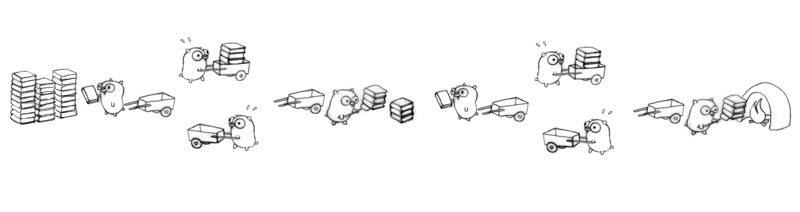
\includegraphics[width=\textwidth]{_figs/busy.jpg}
\end{center}

\end{figure}

Go's concurrency primitives - \textbf{goroutines} and \textbf{channels} - derive from Hoare's Communicating Sequential Processes (CSP.)


Goroutines are like threads: they share memory.


But cheaper:


\begin{itemize}
\item Smaller, segmented stacks.
\item Many goroutines per operating system thread
\end{itemize}


\end{frame}

\begin{frame}[fragile]
\frametitle{fer}


Ok, let's write a \texttt{FairMQ} compatible, inter-operable, toolkit in \myblue{\href{https://golang.org}{\texttt{Go}}}:

	\begin{center}
\myblue{\href{https://github.com/sbinet-alice/fer}{\texttt{github.com/sbinet-alice/fer}}}
	\end{center}

\begin{itemize}
\item create \texttt{fer.Device}
\item create topologies using the same \texttt{JSON} files
\item connect devices via \texttt{ZeroMQ}
\item connect devices via \texttt{nanomsg}
\end{itemize}

All topologies supported by \texttt{FairMQ} should be supported by \texttt{fer} too.

One can mix and match \texttt{C++} and \texttt{Go} devices, see:


\myblue{\href{https://github.com/FairRootGroup/FairRoot/tree/dev/examples/advanced/GoTutorial}{\texttt{github.com/FairRootGroup/FairRoot/tree/dev/examples/advanced/GoTutorial}}}


\end{frame}

\begin{frame}[fragile]
\frametitle{fer - device}


\begin{minted}[fontsize=\small]{go}
import "github.com/sbinet-alice/fer/config"

// Device is a handle to what users get to run via the Fer toolkit.
type Device interface {
	Run(ctl Controler) error
}

\end{minted}

Users need to implement this interface.

\quad\\

Optionally, they may also implement:


\begin{minted}[fontsize=\small]{go}
type DevConfigurer interface {
	Configure(cfg config.Device) error
}
type DevIniter interface {
	Init(ctl Controler) error
}
type DevPauser interface {
	Pause(ctl Controler) error
}
type DevReseter interface {
	Reset(ctl Controler) error
}

\end{minted}


\end{frame}

\begin{frame}[fragile]
\frametitle{fer - controler}


\begin{minted}[fontsize=\small]{go}
// Controler controls devices execution and gives a device access to input and
// output data channels.
type Controler interface {
	Logger
	Chan(name string, i int) (chan Msg, error)
	Done() chan Cmd
}

\end{minted}

\texttt{Controler} is used to give access to input/output channels to the user device.
The \texttt{Done()} channel is used to signal user devices that processing should be somehow interrupted or paused.

\quad\\
Messages and commands are defined as:


\begin{minted}[fontsize=\small]{go}
// Msg is a quantum of data being exchanged between devices.
type Msg struct {
	Data []byte // Data is the message payload.
	Err  error  // Err indicates whether an error occured.
}

// Cmd describes commands to be sent to a device, via a channel.
type Cmd byte

\end{minted}


\end{frame}

\begin{frame}[fragile]

	\begin{columns}
		\begin{column}{0.49\textwidth}
			\begin{block}{}
				\begin{center}
				\texttt{fer} tutorial
				\end{center}
			\end{block}
		\end{column}
	\end{columns}


\end{frame}

\begin{frame}[fragile]
\frametitle{fer - processor}


\begin{minted}[fontsize=\small]{go}
import (
	"github.com/sbinet-alice/fer"
	"github.com/sbinet-alice/fer/config"
)

type processor struct {
	cfg    config.Device
	idatac chan fer.Msg // HL
	odatac chan fer.Msg // HL
}

func (dev *processor) Configure(cfg config.Device) error {
	dev.cfg = cfg
	return nil
}

func (dev *processor) Init(ctl fer.Controler) error {
	idatac, err := ctl.Chan("data1", 0) // handle err // HL
	odatac, err := ctl.Chan("data2", 0) // handle err // HL
	dev.idatac = idatac
	dev.odatac = odatac
	return nil
}

\end{minted}


\end{frame}

\begin{frame}[fragile]
\frametitle{fer - processor}


\begin{minted}[fontsize=\small]{go}
func (dev *processor) Run(ctl fer.Controler) error {
	str := " (modified by "+dev.cfg.Name()+")"
	for {
		select {
		case data := <-dev.idatac: // HL
			out := append([]byte(nil), data.Data...)
			out = append(out, []byte(str)...)
			dev.odatac <- fer.Msg{Data: out} // HL
		case <-ctl.Done():
			return nil
		}
	}
}

func (dev *processor) Pause(ctl fer.Controler) error {
	return nil
}

func (dev *processor) Reset(ctl fer.Controler) error {
	return nil
}

\end{minted}


\end{frame}

\begin{frame}[fragile]
\frametitle{fer - processor}


\begin{minted}[fontsize=\small]{go}
func main() {
	err := fer.Main(&processor{}) // HL
	if err != nil {
		log.Fatal(err)
	}
}

\end{minted}

Build and run like so:



\begin{verbatim}
$> go install ./my-device
$> $GOPATH/bin/my-device --id processor --mq-config ./path-to/config.json

\end{verbatim}


Of course, \texttt{fer} is compatible with \texttt{JSON} files from \texttt{FairMQ}...


More docs:


\myblue{\href{https://godoc.org/github.com/sbinet-alice/fer}{\texttt{godoc.org/github.com/sbinet-alice/fer}}}


\end{frame}

\begin{frame}[fragile]
\frametitle{fer features}


\begin{itemize}
\item \texttt{ZeroMQ} (push/pull, pub/sub, ...), pure-Go \myblue{\href{https://github.com/go-zeromq/zmq4}{\texttt{go-zeromq/zmq4}}}
\item \texttt{nanomsg} (push/pull, pub/sub, ...), pure-Go \myblue{\href{https://github.com/go-mangos/mangos}{\texttt{go-mangos/mangos}}}
\item devices' executables statically compiled, easily cross-compilable
\item \texttt{tcp}, \texttt{inproc} and \texttt{ipc} supported
\item with \texttt{nanomsg}: transport via \texttt{WebSockets} (think: monitoring via a web server)
\item \texttt{FairMQ}-compatible program options
\end{itemize}


\end{frame}

\begin{frame}[fragile]
\frametitle{Conclusions}


\myblue{\href{https://github.com/sbinet-alice/fer}{\texttt{fer}}} is a `FairMQ`-compatible toolkit, written in \myblue{\href{https://golang.org}{\texttt{Go}}}.


Straightforward installation:


\begin{itemize}
\item install \myblue{\href{https://golang.org/doc/install}{\texttt{Go}}} for your platform (macOS, linux, windows, ...)
\item install \myblue{\href{https://github.com/sbinet-alice/fer}{\texttt{fer}}}:
\begin{verbatim}
$> go get github.com/sbinet-alice/fer

\end{verbatim}

\end{itemize}



and voil\`a!

	\begin{exampleblock}{}
\texttt{fer} provides interoperability with \texttt{FairMQ} in a language that is safe, concurrent-friendly, easy to deploy, and ready for the cloud.

\quad

With \texttt{FairMQ} and the microservice-like architecture it enables, one can migrate each device from \texttt{\$LANG1} to \texttt{\$LANG2}, adiabatically.
	\end{exampleblock}


\end{frame}

\begin{frame}[fragile]
\frametitle{Thank you}


	\begin{columns}
		\begin{column}{0.49\textwidth}
	\begin{block}{}
Sebastien Binet\\
CNRS/IN2P3/LPC-Clermont\\
\myblue{\href{https://github.com/sbinet}{\texttt{github.com/sbinet}}}\\
\myblue{\href{https://twitter.com/0xb1ns}{\texttt{@0xbins}}}\\
\myblue{\href{mailto:sebastien.binet@clermont.in2p3.fr}{\texttt{sebastien.binet@clermont.in2p3.fr}}}\\
	\end{block}

\begin{figure}[h]
\begin{center}
\includegraphics[width=1.5cm]{alice-logo.png}
\end{center}

\end{figure}


	\begin{block}{}
Laurent Aphecetche\\
CNRS/IN2P3/Subatech\\
\myblue{\href{https://github.com/aphecetche}{\texttt{github.com/aphecetche}}}\\
\myblue{\href{mailto:laurent.aphecetche@cern.ch}{\texttt{laurent.aphecetche@cern.ch}}}\\
	\end{block}
		\end{column}
	\end{columns}



\end{frame}

\begin{frame}[fragile]

	\begin{columns}
		\begin{column}{0.49\textwidth}
			\begin{exampleblock}{}
				\begin{center}
					Extra material
				\end{center}
			\end{exampleblock}
		\end{column}
	\end{columns}

\end{frame}

\begin{frame}[fragile]
\frametitle{fer non-features}


\begin{itemize}
\item shared-memory "transport": not there yet
\item plugins for the \emph{Dynamic} \emph{Deployment} \emph{System} (\myblue{\href{http://dds.gsi.de/}{\texttt{DDS}}})
\item state machine more limited than FairMQ's
\item no support yet for AliceO2's \emph{Data} \emph{Processing} \emph{Layer} (\myblue{\href{https://github.com/AliceO2Group/AliceO2/tree/dev/Framework/Core}{\texttt{DPL}}}, see \myblue{\href{https://indico.cern.ch/event/587955/timetable/?view=standard\#328-evolution-of-the-alice-sof}{\texttt{\#328}}})
\end{itemize}


\end{frame}

\begin{frame}[fragile]
\frametitle{}


\begin{figure}[h]
\begin{center}
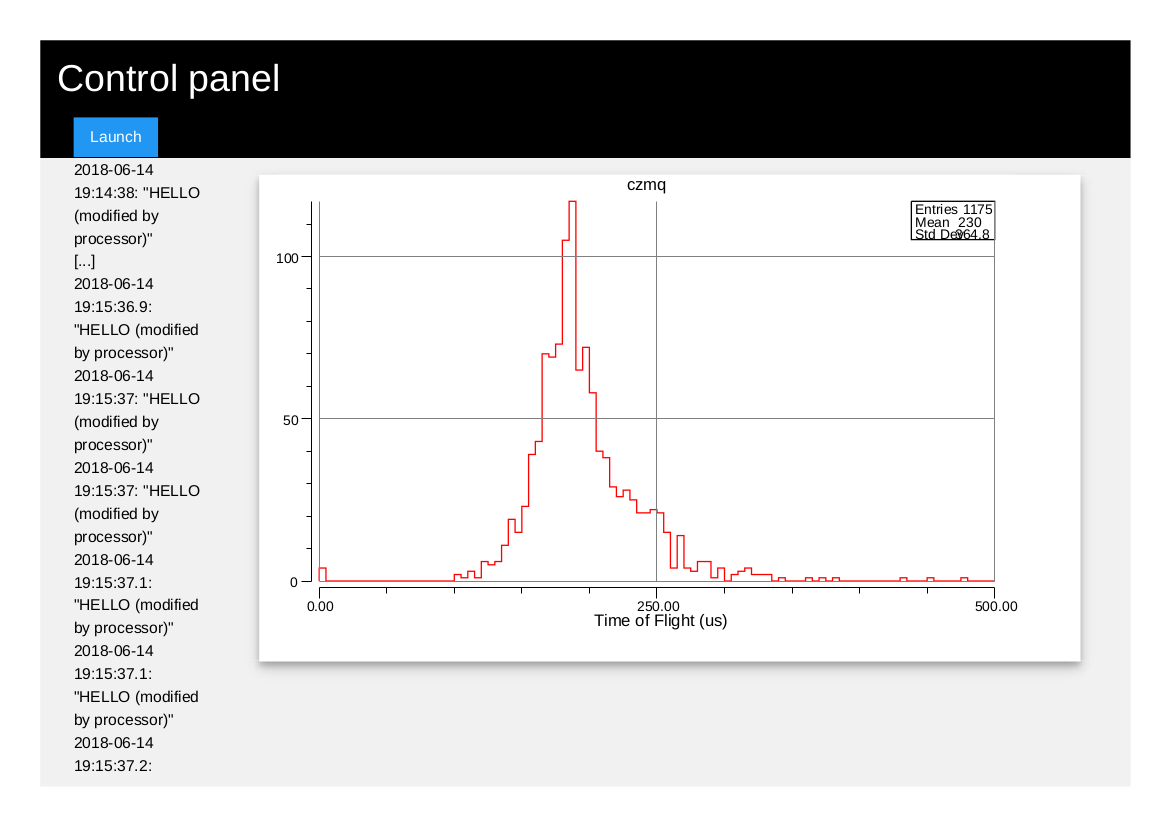
\includegraphics[width=12cm,height=8cm]{_figs/fer-czmq.png}
\end{center}

\end{figure}


\end{frame}

\begin{frame}[fragile]
\frametitle{}


\begin{figure}[h]
\begin{center}
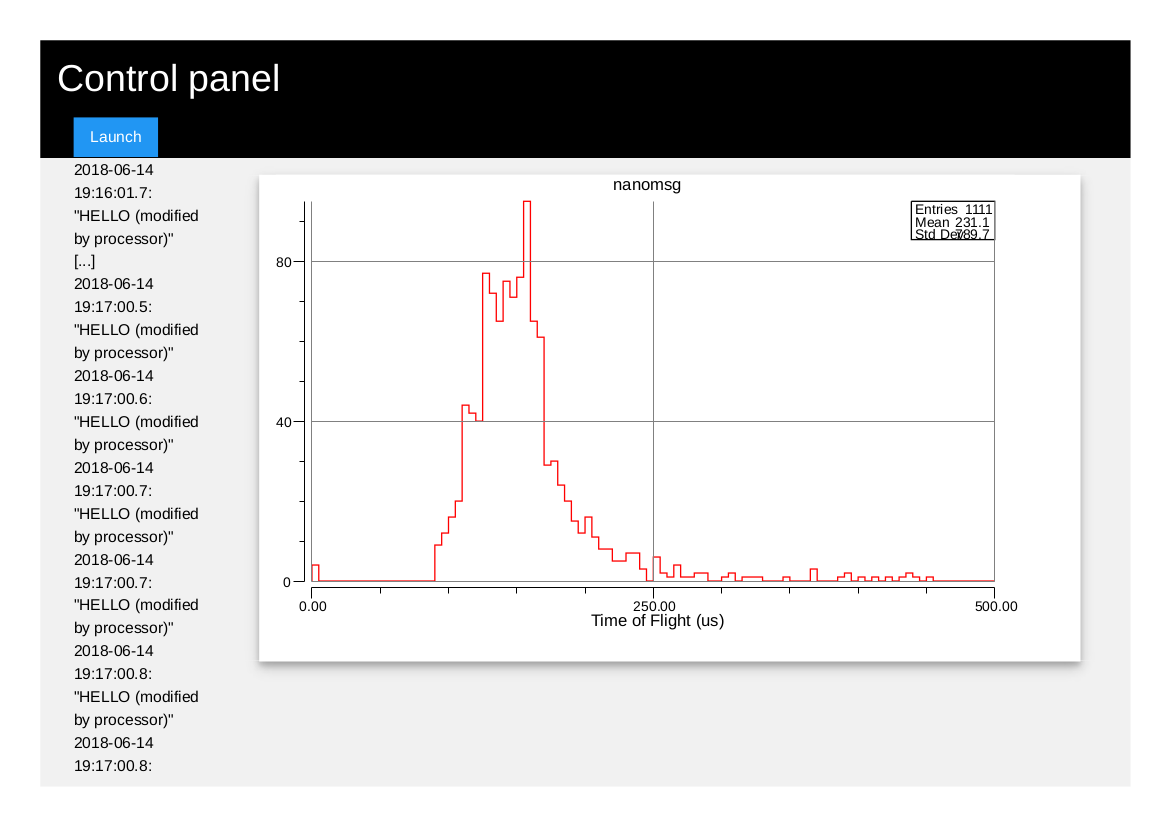
\includegraphics[width=12cm,height=8cm]{_figs/fer-nanomsg.png}
\end{center}

\end{figure}


\end{frame}

\begin{frame}[fragile]
\frametitle{}


\begin{figure}[h]
\begin{center}
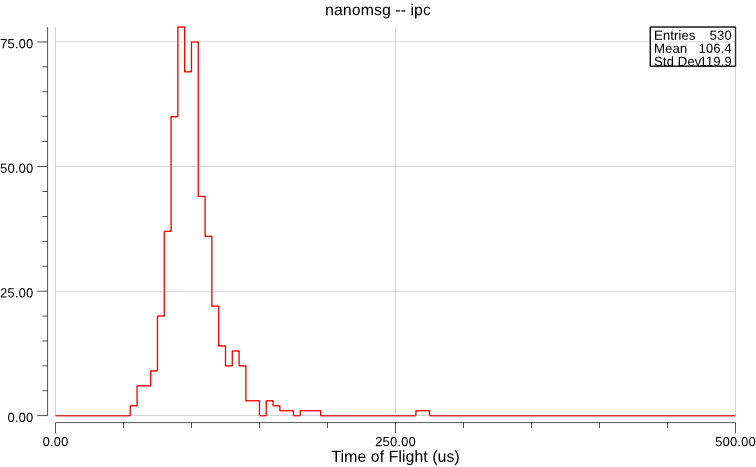
\includegraphics[width=10cm,height=6cm]{_figs/tof-nanomsg-ipc.png}
\end{center}

\end{figure}


\begin{verbatim}
$> ./fer-ex-raw-ctl -timeout=20s -transport=nanomsg -protocol=ipc
real=20.06 user=23.77 sys=17.52 CPU=205% MaxRSS=18808 I/O=0/176

\end{verbatim}



\end{frame}

\begin{frame}[fragile]
\frametitle{}


\begin{figure}[h]
\begin{center}
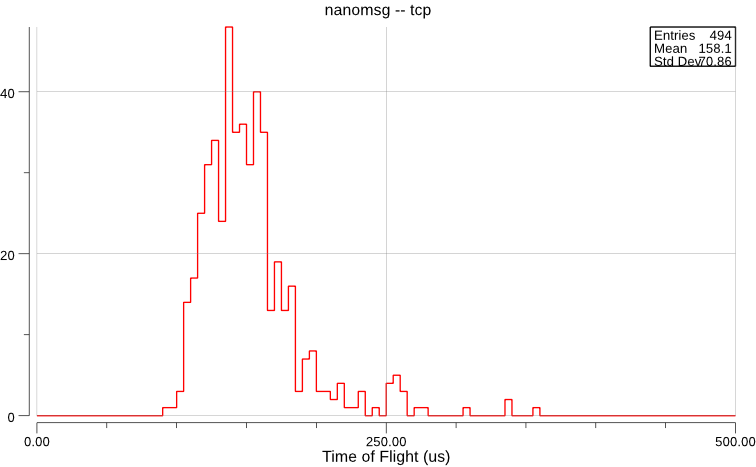
\includegraphics[width=10cm,height=6cm]{_figs/tof-nanomsg-tcp.png}
\end{center}

\end{figure}


\begin{verbatim}
$> ./fer-ex-raw-ctl -timeout=20s -transport=nanomsg -protocol=tcp
real=20.05 user=17.98 sys=24.40 CPU=211% MaxRSS=19548 I/O=0/80

\end{verbatim}



\end{frame}

\begin{frame}[fragile]
\frametitle{}


\begin{figure}[h]
\begin{center}
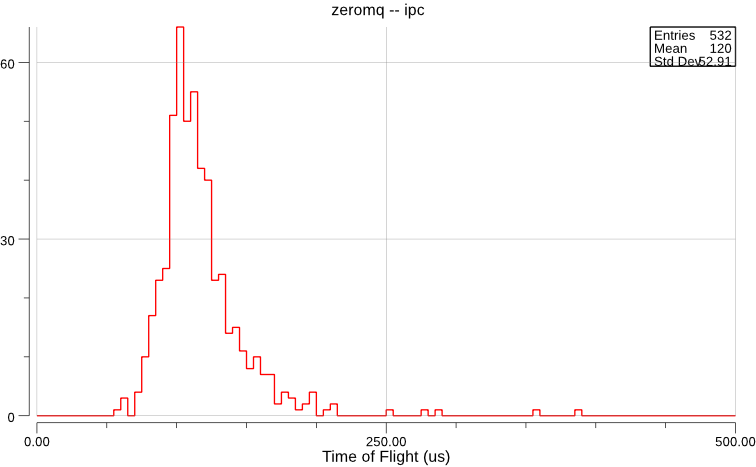
\includegraphics[width=10cm,height=6cm]{_figs/tof-zeromq-ipc.png}
\end{center}

\end{figure}


\begin{verbatim}
$> ./fer-ex-raw-ctl -timeout=20s -transport=zeromq -protocol=ipc
real=20.06 user=27.62 sys=15.63 CPU=215% MaxRSS=19312 I/O=0/80

\end{verbatim}



\end{frame}

\begin{frame}[fragile]
\frametitle{}


\begin{figure}[h]
\begin{center}
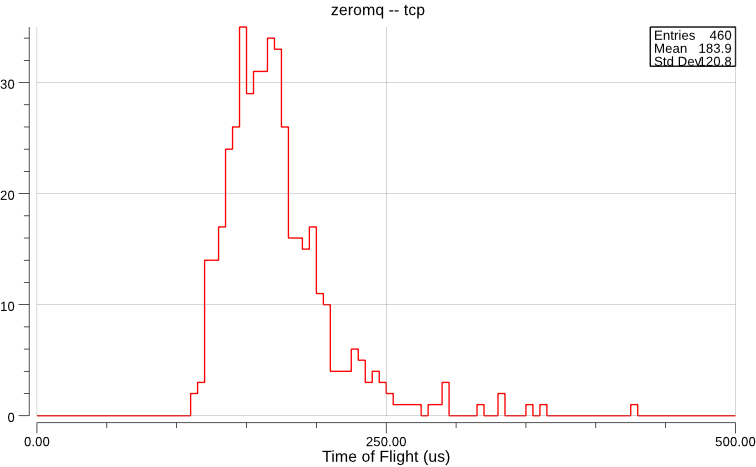
\includegraphics[width=10cm,height=6cm]{_figs/tof-zeromq-tcp.png}
\end{center}

\end{figure}


\begin{verbatim}
$> ./fer-ex-raw-ctl -timeout=20s -transport=zeromq -protocol=tcp
real=20.06 user=21.28 sys=22.28 CPU=217% MaxRSS=19976 I/O=0/80

\end{verbatim}



\end{frame}

\end{document}
